\newsection{Event-Driven Architecture}
\subsection{Description}
The event-driven architecture pattern is a popular distributed asynchronous architecture pattern used to produce highly scalable applications. It is also highly adaptable and can be used for small applications and as well as large, complex ones. The event-driven architecture is made up of highly decoupled, single-purpose event processing components that asynchronously receive and process events. \\
The event-driven architecture pattern consists of two main topologies, the \textbf{mediator} and the \textbf{broker}. The mediator topology is commonly used when you need to orchestrate multiple steps within an event through a central mediator, whereas the broker topology is used when you want to chain events together without the use of a central mediator. 

\subsection{Mediator topology}
The mediator topology is useful for events that have multiple steps and require some level of orchestration to process the event. For example, a single event to place a stock trade might require you to first validate the trade, then check the compliance of that stock trade against various compliance rules, assign the trade to a broker, calculate the commission, and finally place the trade with that broker. All of these steps would require some level of orchestration to determine the order of the steps and which ones can be done serially and in parallel.  \\
There are four main types of architecture components within the mediator topology: \textbf{event queues}, an \textbf{event mediator}, \textbf{event channels}, and \textbf{event processors}. The event flow starts with a client sending an event to an event queue, which is used to transport the event to the event mediator. The event mediator receives the initial event and orchestrates that event by sending additional asynchronous events to event channels to execute each step of the process. Event processors, which listen on the event channels, receive the event from the event mediator and execute specific business logic to process the event.
\Spazio
\begin{figure} [H]
	\centering
	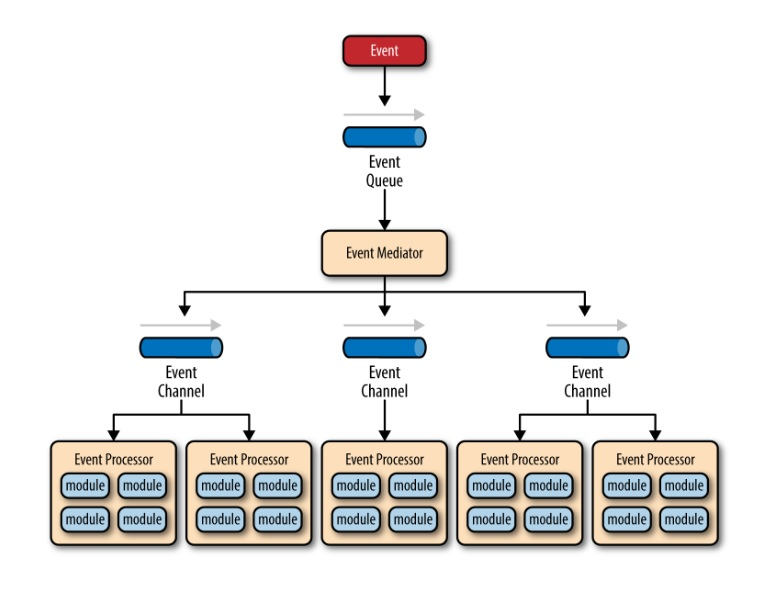
\includegraphics[scale=1]{Img/mediator-topology}
	\caption{Mediator topology architecture}\label{}
\end{figure}

There are two types of events within this pattern: an initial event and a processing event. The initial event is the original event received by the mediator, whereas the processing events are ones that are generated by the mediator and received by the event-processing components.

\subsubsection{Event-mediator}
The event-mediator component is responsible for orchestrating the steps contained within the initial event. For each step in the initial event, the event mediator sends out a specific processing event to an event channel, which is then received and processed by the event processor. It is important to note that the event mediator doesn't actually perform the business logic necessary to process the initial event; rather, it knows of the steps required to process the initial event.

\subsubsection{Event channels}
Event channels are used by the event mediator to asynchronously pass specific processing events related to each step in the initial event to the event processors. The event channels can be either message queues or message topics, although message topics are most widely used with the mediator topology so that processing events can be processed by multiple event processors(each performing a different task based on the processing event received).

\subsubsection{Event processor}
The event processor components contain the application business logic necessary to process the processing event. Event processors are self-contained, independent, highly decoupled architecture components that perform a specific task in the application or system. While the granularity of the event-processor component can vary from fine-grained (e.g. calculate sales tax on an order) to coarse-grained (e.g. process an insurance claim), it is important to keep in mind that in general, each event-processor component should perform a single business task and not rely on other event processors to complete its specific task.

\subsubsection{Event queue}
It is common to have anywhere from a dozen to several hundred event queues in an event-driven architecture. The pattern does not specify the implementation of the event queue component; it can be a message queue, a web service endpoint or any combination thereof.

\subsection{Broker topology}
The broker topology differs from the mediator topology in that there is no central event mediator; rather, the message flow is distributed across the event processor components in a chain-like fashion through a lightweight message broker. This topology is useful when you have a relatively simple event processing flow. \\
There are two main types of architecture components: a \textbf{broker} component and an \textbf{event processor} component. The broker component can be centralized or federated and contains all of the event channels that are used within the event flow. The event channels contained within the broker component can be message queues, message topics, or a combination of both.

\begin{figure} [H]
	\centering
	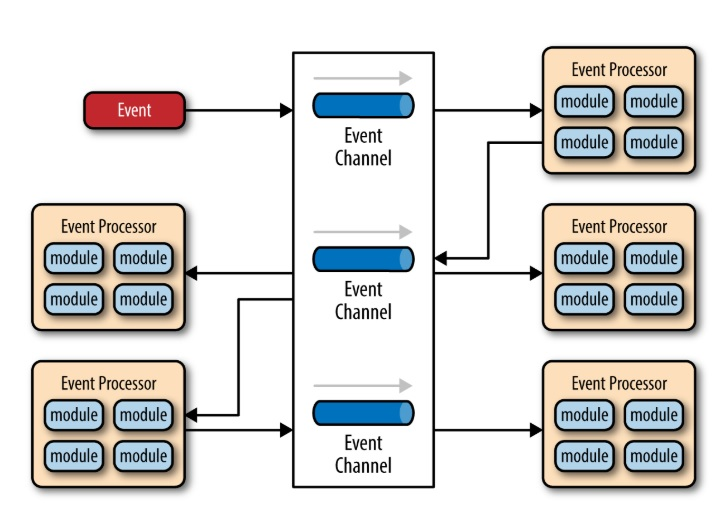
\includegraphics[scale=1]{Img/broker-topology}
	\caption{Broker topology architecture}\label{}
\end{figure}

There is no central event-mediator component controlling and orchestrating the initial event; rather, each event-processor component is responsible for processing an event and publishing a new event indicating the action it just performed. \\
The broker topology is all about the chaining of events to perform a business function; once an event processor hands off the event, it is no longer involved with the processing of that specific event.


